\documentclass[a4paper, fontsize=11pt]{scrartcl} % A4 paper and 11pt font 
\usepackage[a4paper,left=3cm,right=2cm,top=2.5cm,bottom=2.5cm]{geometry}

\usepackage[T1]{fontenc} % Use 8-bit encoding that has 256 glyphs
%\usepackage{fourier} % Use the Adobe Utopia font for the document - comment this line to return to the LaTeX default
\usepackage[spanish]{babel} % Spanish language/hyphenation
\selectlanguage{spanish}
\usepackage[utf8]{inputenc}
\usepackage{amsmath,amsfonts,amsthm} % Math packages
\usepackage{graphicx} % The graphicx package
\usepackage{placeins}
\usepackage{caption}
\usepackage{subcaption}

\usepackage{cite} % para contraer referencias


\usepackage{listings} % Insert Scripts
\usepackage{color} %red, green, blue, yellow, cyan, magenta, black, white
\definecolor{mygreen}{RGB}{28,172,0} % color values Red, Green, Blue
\definecolor{mylilas}{RGB}{170,55,241}

\lstset{language=Matlab,%
	%basicstyle=\color{red},
	breaklines=true,%
	morekeywords={matlab2tikz},
	keywordstyle=\color{blue},%
	morekeywords=[2]{1}, keywordstyle=[2]{\color{black}},
	identifierstyle=\color{black},%
	stringstyle=\color{mylilas},
	commentstyle=\color{mygreen},%
	showstringspaces=false,%without this there will be a symbol in the places where there is a space
	numbers=left,%
	numberstyle={\tiny \color{black}},% size of the numbers
	numbersep=9pt, % this defines how far the numbers are from the text
	emph=[1]{for,end,break},emphstyle=[1]\color{red}, %some words to emphasise
	%emph=[2]{word1,word2}, emphstyle=[2]{style},    
}

\usepackage{sectsty} % Allows customizing section commands
%\allsectionsfont{\centering \normalfont\scshape} % Make all sections centered, the default font and small caps

\usepackage{fancyhdr} % Custom headers and footers
\pagestyle{fancyplain} % Makes all pages in the document conform to the custom headers and footers
\fancyhead{} % No page header - if you want one, create it in the same way as the footers below
\fancyfoot[L]{} % Empty left footer
\fancyfoot[C]{} % Empty center footer
\fancyfoot[R]{\thepage} % Page numbering for right footer
\renewcommand{\headrulewidth}{0pt} % Remove header underlines
\renewcommand{\footrulewidth}{0pt} % Remove footer underlines
\setlength{\headheight}{13.6pt} % Customize the height of the header

\numberwithin{equation}{section} % Number equations within sections (i.e. 1.1, 1.2, 2.1, 2.2 instead of 1, 2, 3, 4)
\numberwithin{figure}{section} % Number figures within sections (i.e. 1.1, 1.2, 2.1, 2.2 instead of 1, 2, 3, 4)
\numberwithin{table}{section} % Number tables within sections (i.e. 1.1, 1.2, 2.1, 2.2 instead of 1, 2, 3, 4)

%\setlength\parindent{0pt} % Removes all indentation from paragraphs - comment this line for an assignment with lots of text

\newenvironment{myalign}{\par\nobreak\large\noindent\align}{\endalign} %Altering fontsize in equations globally

%----------------------------------------------------------------------------------------
%	TITLE SECTION
%----------------------------------------------------------------------------------------

\newcommand{\horrule}[1]{\rule{\linewidth}{#1}} % Create horizontal rule command with 1 argument of height

\title{	
	\normalfont \normalsize 
	\textsc{Máster en Automática y Robótica - UPM} \\ [25pt] % Your university, school and/or department name(s)
	\horrule{0.5pt} \\[0.4cm] % Thin top horizontal rule
	\huge Trabajo 1a de Cinemática de Robots \\ % The assignment title
	\horrule{2pt} \\[0.5cm] % Thick bottom horizontal rule
}

\author{Jorge Camarero Vera - 07052} % Your name

\date{\normalsize\today} % Today's date or a custom date

\begin{document}
	\maketitle
	
	\section{Explicación de la tarea}
	
	Desarrollar una función en Matlab con las siguientes especificaciones:
	
	\begin{enumerate}
		\item Recibirá como dato los parámetros de DH de un robot de un mínimo de 2 y un máximo de 7 gdl.
		\item Permitirá definir los valores de las coordenadas articulares. Estos podrán variarse mediante sliders. En caso de grados de libertad de rotación, las unidades serán grados sexagesimales.
		\item Representará los valores de localización del extremo del robot en el espacio de la tarea pudiéndose escoger (mediante un botón de selección) entre:
		\begin{itemize}
			\item Posición del extremo en coordenadas cartesianas (XYZ) y ángulos de Euler WUW.
			\item Matriz de Transformación Homogénea del extremo.
		\end{itemize}
		\item Representará en "alambres" al robot en las coordenadas indicadas.
	\end{enumerate}
	
	%\begin{figure}[h!]
	%	\centering
	%	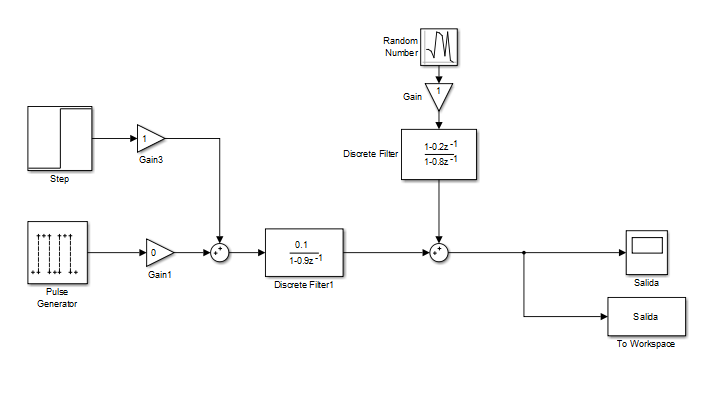
\includegraphics[width=1.0\linewidth]{images/Original_System.PNG}
	%	\caption{Modelo inicial}
	%	\label{Modelo Inicial}
	%\end{figure}
	%\FloatBarrier
	
	\section{Desarrolo del Programa}
	
	Se ha creado una interfaz gráfica, GUI, para manejar las entradas y salidas que se piden para la realización de este trabajo. La GUI se ha dividido en cuatro paneles y un plot para representar el robot. Estos cuatro paneles son:
	
	\begin{itemize}
		\item Parámetros de Denavid-Hartenberg
		\item Configuraciones del Robot
		\item Rotaciones
		\item Coordenadas de la herramienta
	\end{itemize}
	
	\subsection{Parámetros de Denavid-Hartenberg}
	
	En este panel, Figura \ref{Parametros}, hay una tabla para introducir los parámetros de DH, un botón para establecer los grados de libertad de la tabla anterior, una pestaña para seleccionar si se desean introducir los parámetros que implicar rotaciones en grados o en radianes, otra pestaña para establecer parámetros de DH de robots ya predefinidos. Por último se encuentra el botón de calcular que permite obtener a partir de los parámetros introducidos y las rotaciones dadas, el plot del robot y las coordenadas de las herramientas y/o su matriz homogénea.\\
	
	\begin{figure}[h!]
		\centering
		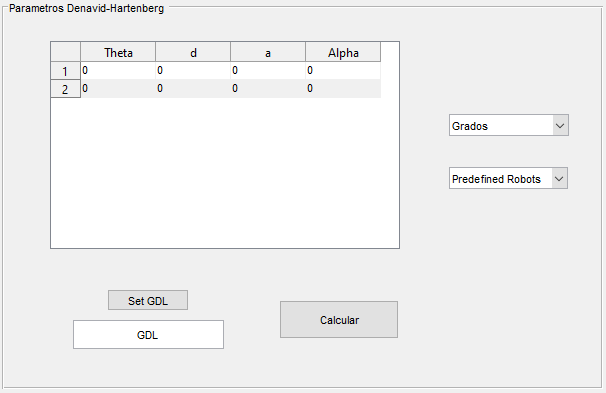
\includegraphics[width=0.8\linewidth]{images/Param.PNG}
		\caption{Panel por defecto de Parámetros de Denavid-Hartenberg}
		\label{Parametros}
	\end{figure}
	\FloatBarrier
	
	La tabla para escribir los parámetro de DH por defecto viene para 2 gdl, pero se puede cambiar abajo estableciendo los GDL que uno quiera desde 0 hasta infinito (probado hasta 1 millón), Figura \ref{Parametros_Inf}. Por lo que así conseguimos abrir el camino para representar robots sobreactuados por encima de 7 gdl.\\
	
	\begin{figure}[h!]
		\centering
		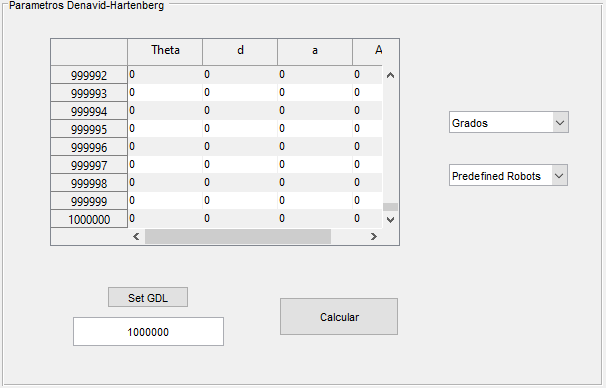
\includegraphics[width=0.8\linewidth]{images/Param_Inf.PNG}
		\caption{Panel de Parámetros de Denavid-Hartenberg con 1 millón de GDL}
		\label{Parametros_Inf}
	\end{figure}
	\FloatBarrier
	
	A la hora de ir probando la interfaz era incómodo estar cargando a mano una y otra vez los parámetros de los robots, por lo que se creó la pestaña con distintos robots predefinidos para ir probando, la lista abarca robots que se encuentran dentro de la toolbox de robótica, pero en el código los parámetros de DH los he escrito a mano, por lo que sólo han tenido que ser escritos una vez. Esto aporta ventajas de cara a la depuración del código y del uso del programa, ya que se cargan robots ya existentes, y por tanto podemos trabajar con ellos sin tener que conocer de antemano sus parámetros de DH.\\
	
	En el ejercicio se pedía para las rotaciones que los datos se introdujeran en grados sexagesimales, como desconocía si se refería también a la tabla de parámetros de DH, ha sido creada una pestaña para seleccionar si se quieren introducir los parámetros rotacionales en grados o radianes. Si se selecciona un robot predefinido habrá que establecer la pestaña en radianes, ya que estos se establecen en la tabla en radianes.\\
	
	Sobre la tabla para introducir los parámetros de DH, como se ve en la Figura \ref{Parametros}, no aparece el offset típico de la función \textit{Link} de la toolbox de robótica. Esto lo he solucionado introduciendo los parámetros de manera natural como se ha explicado en clase, Figura \ref{Parametros_DH}. Esto se consigue haciendo que la tabla reciba los parámetros como \textit{strings} y mediante expresiones regulares ir separando unas partes de otras y mover ambas partes a donde se corresponden en la función \textit{Link} de la toolbox de robótica. Vemos que también se puede escribir números como \textit{pi}.\\
	
	\begin{figure}[h!]
		\centering
		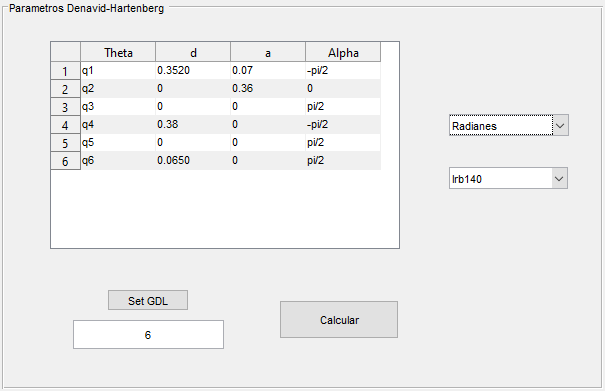
\includegraphics[width=0.8\linewidth]{images/Param_DH.PNG}
		\caption{Panel de Parámetros de Denavid-Hartenberg con datos introducidos}
		\label{Parametros_DH}
	\end{figure}
	\FloatBarrier
	
	A la hora de presionar el botón calcular para obtener los datos requeridos emplea los parámetros de DH que hemos dado, las rotaciones introducidas y las configuraciones del robot, estos dos últimos se explica en los siguientes apartados.\\
	
	\subsection{Rotaciones}
	
	Las rotaciones, de 1 a 7, se introducen en grados sexagesimales o bien mediante los \textit{sliders}, van de -180º a 180º, o bien mediante la tabla presente en el panel, Figura \ref{Rotaciones}. Al introducir los datos en la table automáticamente se mueven los \textit{sliders} y viceversa. Si los gdl que se introducen para el robot son inferiores al número de rotaciones introducidas el programa ignorará las rotaciones sobrantes.\\
	
	\begin{figure}[h!]
		\centering
		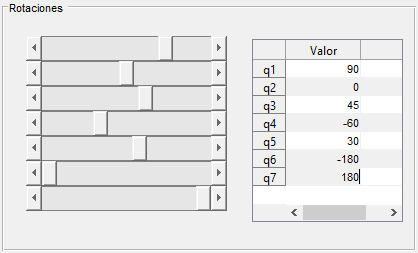
\includegraphics[width=0.6\linewidth]{images/Rotaciones.PNG}
		\caption{Panel de Rotaciones}
		\label{Rotaciones}
	\end{figure}
	\FloatBarrier
	
	\subsection{Configuraciones del Robot}
	
	En el panel de configuraciones del robot, Figura \ref{Configuraciones}, se pueden introducir matrices homogéneas de la herramienta y la base, para desplazar el origen o rotarlo, además de vector de gravedad. Aunque esto explícitamente no se pedía para este trabajo lo he introducido ya que ciertos robots predefinidos tenían modificados estos parámetros, y se decidió incluirlo en la GUI.\\
	
	\begin{figure}[h!]
		\centering
		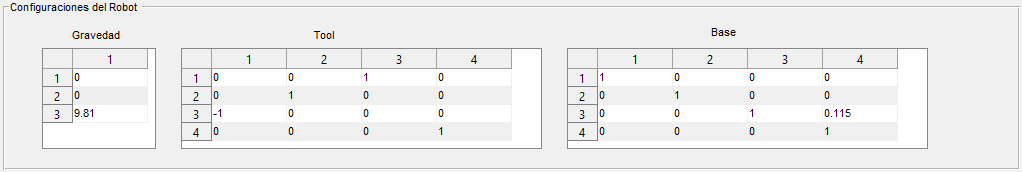
\includegraphics[width=1.0\linewidth]{images/Config.PNG}
		\caption{Panel de Configuraciones del Robot. Con los datos del robot P8 de 8 gdl y modificación extra de la posición de la base.}
		\label{Configuraciones}
	\end{figure}
	\FloatBarrier
	
	\subsection{Coordenadas de la Herramienta}
	
	En este trabajo se pide representar los valores de localización del extremo del robot en el espacio de la tarea pudiéndose escoger (mediante un botón de selección) entre:
	
	\begin{itemize}
		\item Posición del extremo en coordenadas cartesianas (XYZ) y ángulos de Euler WUW.
		\item Matriz de Transformación Homogénea del extremo.
	\end{itemize}
	
	Para completar esta tarea se ha creado una pestaña para seleccionar la salida deseada, y estos datos salen por una de las dos tablas, la de la izquierda para la posición del extremo en coordenadas cartesianas (XYZ) y ángulos de Euler WUW, y la de la derecha para la matriz de transformación homogénea del extremo, Figura \ref{Output}.\\
	
	\begin{figure}[h!]
		\centering
		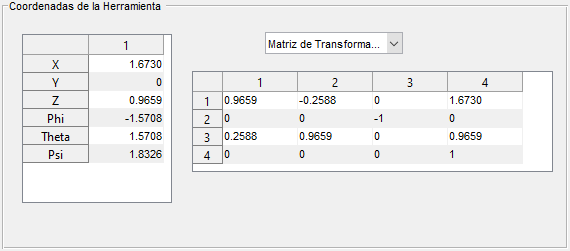
\includegraphics[width=0.8\linewidth]{images/Output.PNG}
		\caption{Panel de Coordenadas de la Herramienta.}
		\label{Output}
	\end{figure}
	\FloatBarrier
	
	Estos resultados se obtienen automáticamente al pulsar el botón \textbf{Calcular} en el panel de parámetros Denavid-Hartenberg. Si primero se selecciona las coordenadas y se pulsa calcular, y después se selecciona la matriz de transformación homogénea y se vuelve a calcular se mantienen los resultados en ambas tablas.\\
	
	\subsection{Plot del Robot}
	
	Al pulsar el botón \textbf{Calcular} también se genera un plot en tres dimensiones en el que se muestra el robot en la posición calculada, Figura \ref{Plot}.
	
	\begin{figure}[h!]
		\centering
		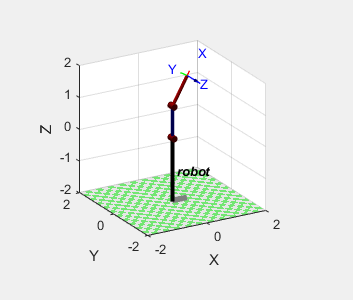
\includegraphics[width=0.6\linewidth]{images/Plot.PNG}
		\caption{Plot en 3D de la posición calculada de un robot con 2 gdl.}
		\label{Plot}
	\end{figure}
	\FloatBarrier
	
	\section{Pruebas hechas con distintos robots y grados de libertad}
	
	Se han hecho pruebas para el correcto funcionamiento de la GUI que van desde robots de 1 gdl, Figura \ref{GDL1}, hasta 8 gdl, Figuras \ref{GDL8} y \ref{GDL8_J}, éste último presenta GDL tanto rotacionales como prismáticos. Pese a que los parámetros de DH se introducen en radiantes para introducir las rotaciones se deberán hacer en grados sexagesimales, Figura \ref{GDL3}.
	
	\begin{figure}[h!]
		\centering
		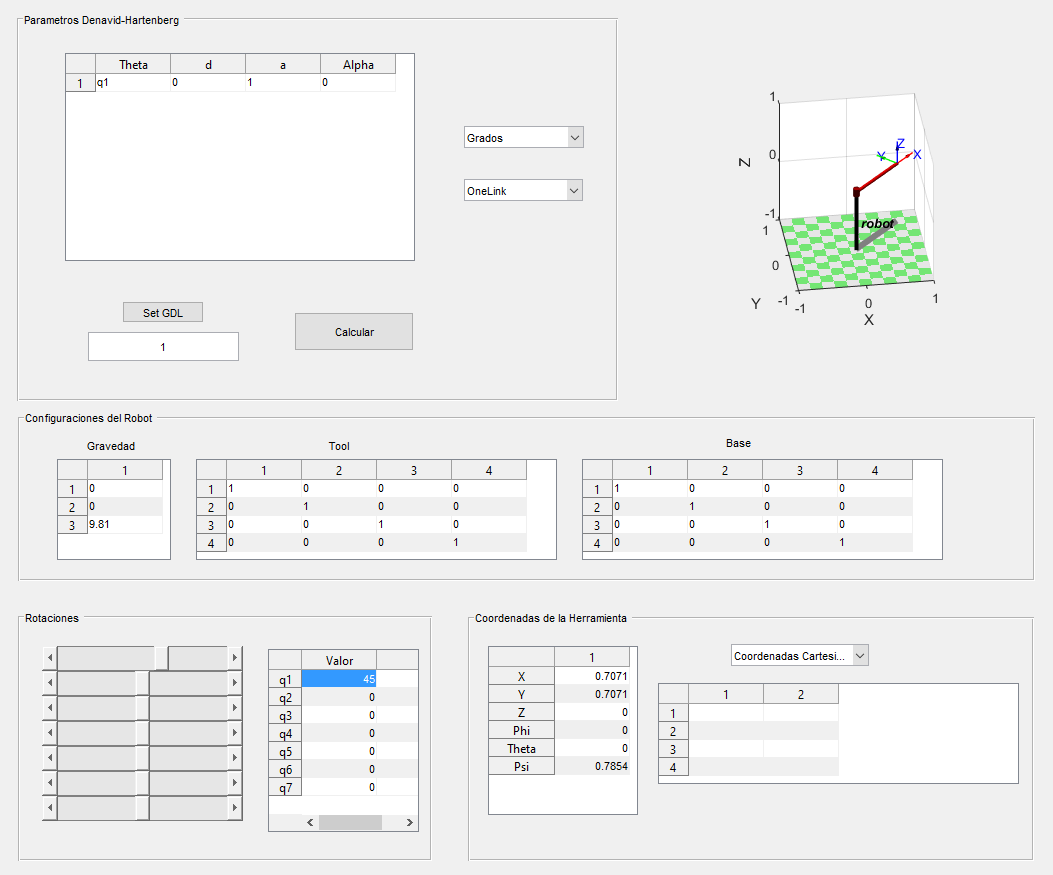
\includegraphics[width=1.0\linewidth]{images/GDL1.PNG}
		\caption{GUI presentando los datos de un robot con 1 gdl.}
		\label{GDL1}
	\end{figure}
	\FloatBarrier
	
	\begin{figure}[h!]
		\centering
		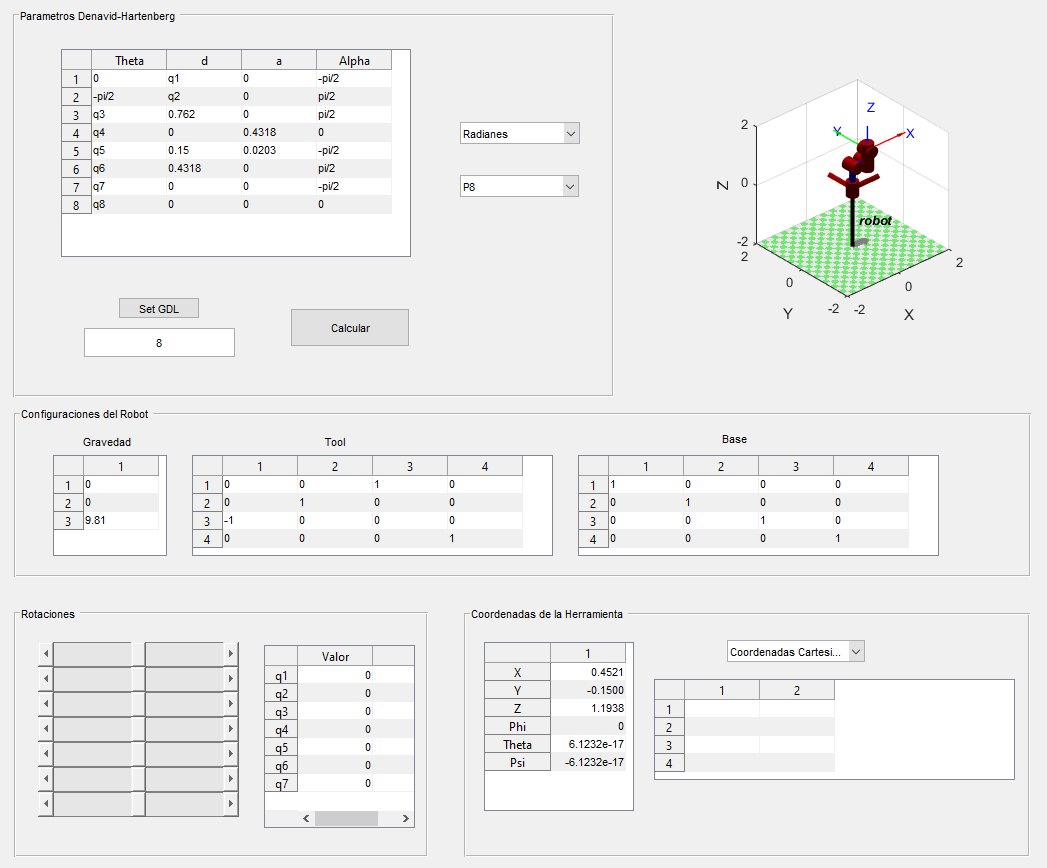
\includegraphics[width=1.0\linewidth]{images/GDL8.PNG}
		\caption{GUI presentando los datos de un robot con 8 gdl, es el robot predefinido \textit{P8}.}
		\label{GDL8}
	\end{figure}
	\FloatBarrier
	
	\begin{figure}[h!]
		\centering
		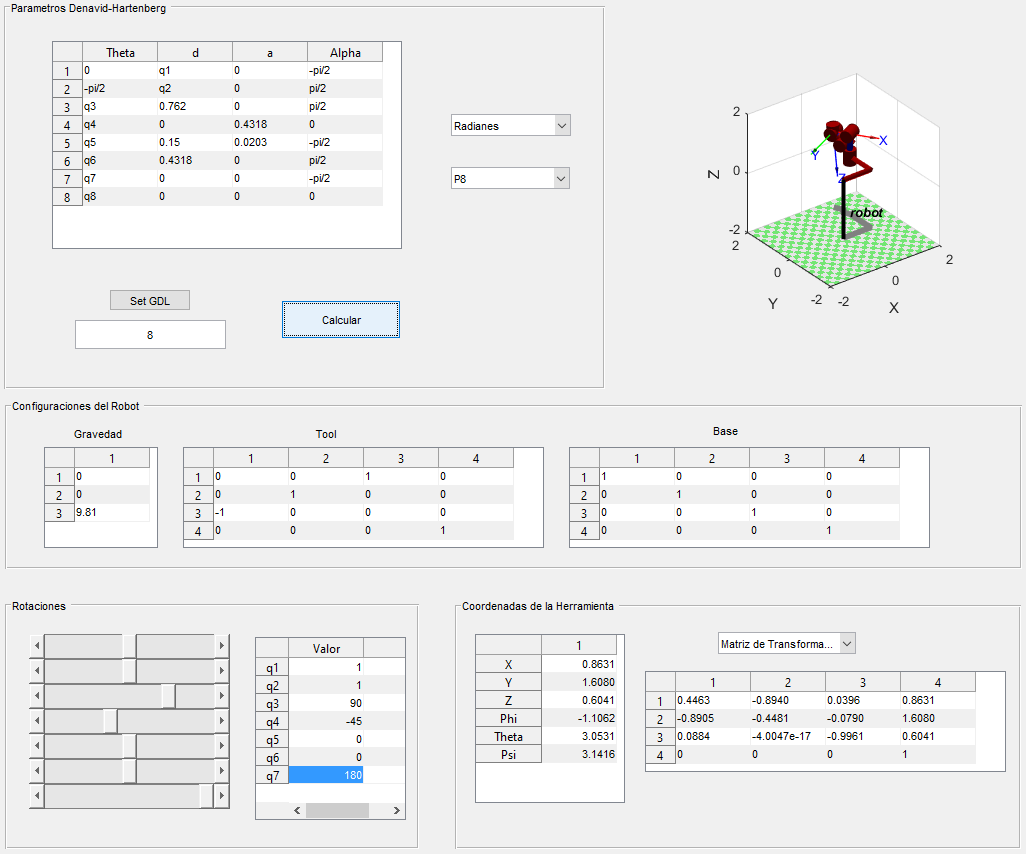
\includegraphics[width=1.0\linewidth]{images/GDL8_J.PNG}
		\caption{GUI presentando los datos de un robot con 8 gdl, es el robot predefinido \textit{P8}. Se han establecido rotaciones y movimientos en gdl prismáticos.}
		\label{GDL8_J}
	\end{figure}
	\FloatBarrier
	
	\begin{figure}[h!]
		\centering
		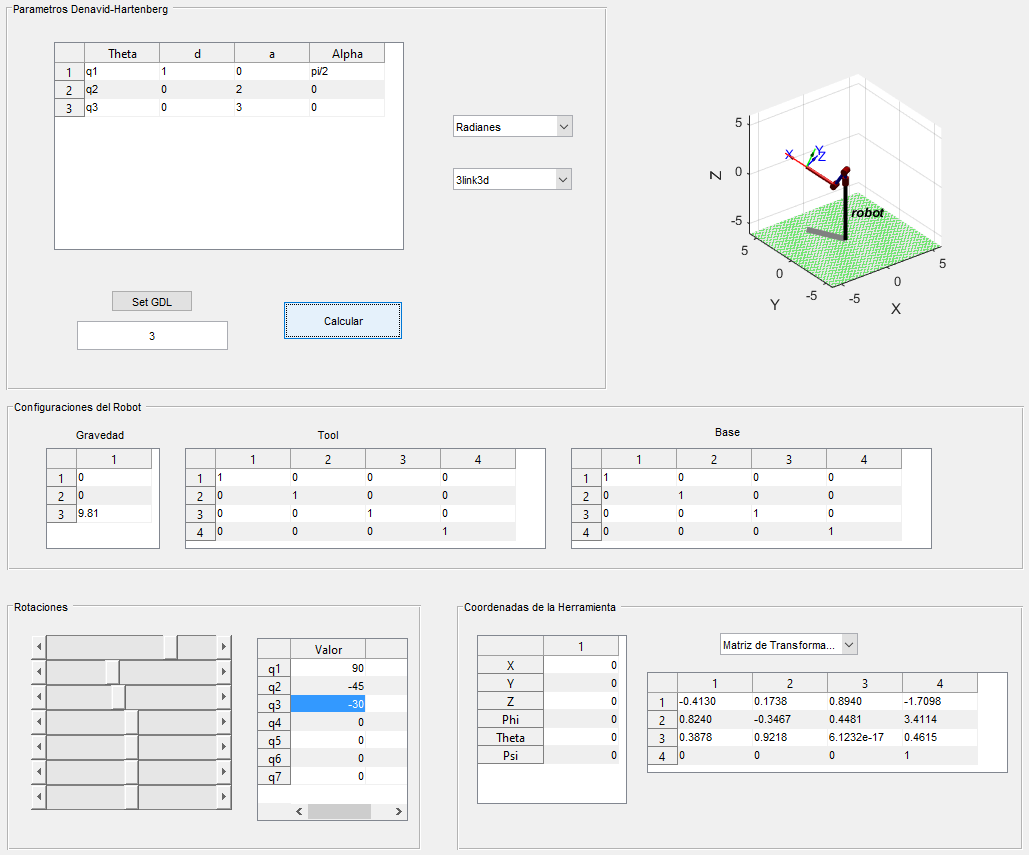
\includegraphics[width=1.0\linewidth]{images/GDL3.PNG}
		\caption{GUI presentando los datos de un robot con 3 gdl. Las rotaciones son en grados sexagesimales y se pide calcular la matriz de transformación homogénea.}
		\label{GDL3}
	\end{figure}
	\FloatBarrier
	
	\section{Planteamientos al Futuro}
	
	A lo largo de la escritura del código me han surgido errores o problemas que por falta de tiempo o quedar fuera del alcance de este trabajo no he llegado a hacer.\\
	
	Un problema es que al hacer \textit{plot} del robot con la toolbox ancla la GUI en la parte superior de la pantalla impidiendo mover esta por la pantalla. Esto no he podido solucionarlo al tratarse de un bug del código de la toolbox y no he tenido tiempo de depurarlo.\\
	
	Otro problema que surge con el mismo \textit{plot} es que si tienes coordenadas prismáticas y haces \textit{plot} surge un error, que se soluciona al darle los límites del volumen del \textit{workspace}, de momento lo mantengo fijo en [-2 2 -2 2 -2 2], pero de cara al siguiente trabajo he pensado modificarlo dinámicamente en función de la posición de la herramienta u otros parámetros, el problema de emplear la posición de la herramienta es que no tiene porqué ser la parte más alejada del robot. Otra solución es la suma de ciertos parámetros prismáticos de DH y emplearlos para delimitar el \textit{workplace}.\\
	
	Otra opción que me gustaría implementar es que al cargar un robot predefinido se puedan establecer con parámetros rotativos de DH en grados sexagesimales.\\
	
	Pero la principal tarea extra que intentaré implementar en el trabajo 1b es la generación dinámica de los \textit{sliders} de rotaciones en función de los gdl establecidos. Así se podrá controlar todas las rotaciones de un robot de más de 7 grados de libertad, que es el máximo que se puede actualmente.\\

	También seguiría introduciendo nuevos robots predefinidos e incluso poder incluir múltiples robots a la vez en los cálculos, por ejemplo el robot \textit{Baxter} está formado por dos robots (brazos) independientes, el izquierdo y el derecho. Sería muy interesante poder incluir esta opción.\\
	
	\bibliographystyle{acm} % estilo de la bibliografía.
	\bibliography{yyyy} 
	
	\begin{thebibliography}{X}
		
		\bibitem{ToolBoxRobotic} \textsc{Peter Corke} \textit{Robotics, Vision and Control. Fundamental Algorithms in Matlab}, Springer Tracs in Advanced Robotics.
		
		
	\end{thebibliography}
	
\end{document}